\chapter{Motivation, and introduction to graph theory}

\section{Aspects of Networks}
\subsection{Overview: The Connected World}
A network is a fundamentally defined as a pattern of interconnections among a set of objects. There has been a rising public interest in the complex ``connectedness of modern society'', driven by this idea. 

\paragraph{Areas where network appear}

\begin{enumerate}[nosep]
    \item Social networks: collections of social ties (e.g., friendships, business relationships) have increased in complexity due to technological advances like global communication and digital interaction, weakening traditional geographic limitations. 
    \item Information networks: the information consumed by people has a networked structure. Understanding any piece of information requires knowing how it refers to or is endorsed by other pieces within a large network of links.
    \item Technological and economic systems: these systems rely on networks of enormous complexity, making their behavior hard to predict and susceptible to disruptions that can spread, turning localized breakdowns into cascading failures or financial crises.
    \item Operational networks: many organizations depend on complex networks of people, resources, and processes to function effectively. Understanding and optimizing these networks is crucial for efficiency and resilience. Examples include networks of suppliers for global manufacturing, networks of users for websites, and networks of advertisers for media companies.
\end{enumerate}
\begin{figure}[ht]
\centering

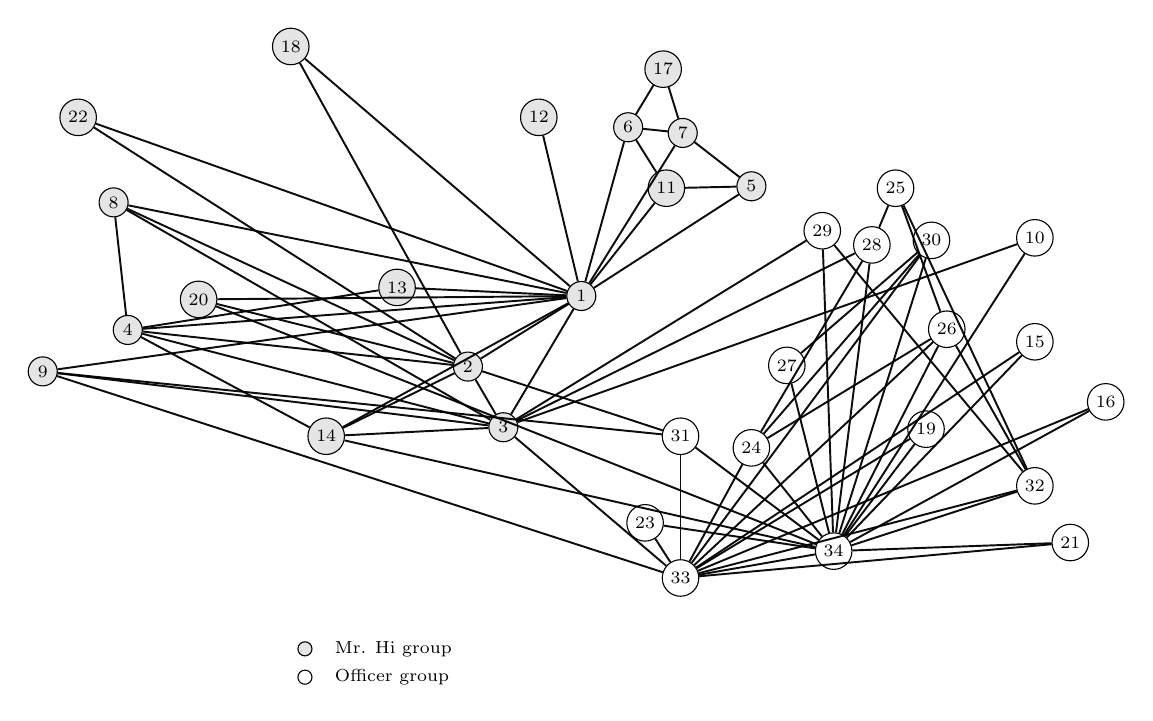
\begin{tikzpicture}[
  xscale=0.9, yscale=0.9, transform shape,
  hi/.style={circle, draw=black, fill=gray!20, inner sep=2.0pt, font=\scriptsize},
  off/.style={circle, draw=black, fill=white,   inner sep=2.0pt, font=\scriptsize},
  e/.style={line width=0.7pt, draw=black, opacity=0.95}
]

% (x and y stretched; coordinates updated directly)
\coordinate (p1) at (4.6,4.479);
\coordinate (p2) at (3,3.483);
\coordinate (p3) at (3.5,2.627);
\coordinate (p4) at (-1.8,4);
\coordinate (p5) at (7,6.027);
\coordinate (p6) at (5.261,6.860);
\coordinate (p7) at (6.031,6.780);
\coordinate (p8) at (-2,5.8);
\coordinate (p9) at (-3,3.415);
\coordinate (p10) at (11,5.3);
\coordinate (p11) at (5.8,6);
\coordinate (p12) at (4,7);
\coordinate (p13) at (2,4.6);
\coordinate (p14) at (1,2.5);
\coordinate (p15) at (11,3.833);
\coordinate (p16) at (12,2.985);
\coordinate (p17) at (5.755,7.680);
\coordinate (p18) at (0.5,8);
\coordinate (p19) at (9.464,2.6);
\coordinate (p20) at (-0.8,4.431);
\coordinate (p21) at (11.5,1);
\coordinate (p22) at (-2.5,7);
\coordinate (p23) at (5.5,1.278);
\coordinate (p24) at (7,2.336);
\coordinate (p25) at (9.034,6);
\coordinate (p26) at (9.757,4.010);
\coordinate (p27) at (7.5,3.5);
\coordinate (p28) at (8.7,5.2);
\coordinate (p29) at (8,5.4);
\coordinate (p30) at (9.541,5.264);
\coordinate (p31) at (6,2.5);
\coordinate (p32) at (11,1.8);
\coordinate (p33) at (6,0.500);
\coordinate (p34) at (8.161,0.879);



% --- Nodes (Mr. Hi vs Officer) ---
% Mr. Hi club: 1,2,3,4,5,6,7,8,9,11,12,13,14,17,18,20,22
\node[hi]  (p1)  at (p1)  {1};
\node[hi]  (p2)  at (p2)  {2};
\node[hi]  (p3)  at (p3)  {3};
\node[hi]  (p4)  at (p4)  {4};
\node[hi]  (p5)  at (p5)  {5};
\node[hi]  (p6)  at (p6)  {6};
\node[hi]  (p7)  at (p7)  {7};
\node[hi]  (p8)  at (p8)  {8};
\node[hi]  (p9)  at (p9)  {9};
\node[off] (p10) at (p10) {10};
\node[hi]  (p11) at (p11) {11};
\node[hi]  (p12) at (p12) {12};
\node[hi]  (p13) at (p13) {13};
\node[hi]  (p14) at (p14) {14};
\node[off] (p15) at (p15) {15};
\node[off] (p16) at (p16) {16};
\node[hi]  (p17) at (p17) {17};
\node[hi]  (p18) at (p18) {18};
\node[off] (p19) at (p19) {19};
\node[hi]  (p20) at (p20) {20};
\node[off] (p21) at (p21) {21};
\node[hi]  (p22) at (p22) {22};
\node[off] (p23) at (p23) {23};
\node[off] (p24) at (p24) {24};
\node[off] (p25) at (p25) {25};
\node[off] (p26) at (p26) {26};
\node[off] (p27) at (p27) {27};
\node[off] (p28) at (p28) {28};
\node[off] (p29) at (p29) {29};
\node[off] (p30) at (p30) {30};
\node[off] (p31) at (p31) {31};
\node[off] (p32) at (p32) {32};
\node[off] (p33) at (p33) {33};
\node[off] (p34) at (p34) {34};

% --- Edges (undirected) ---
\path[e] (p1) -- (p2);
\path[e] (p1) -- (p3);
\path[e] (p1) -- (p4);
\path[e] (p1) -- (p5);
\path[e] (p1) -- (p6);
\path[e] (p1) -- (p7);
\path[e] (p1) -- (p8);
\path[e] (p1) -- (p9);
\path[e] (p1) -- (p11);
\path[e] (p1) -- (p12);
\path[e] (p1) -- (p13);
\path[e] (p1) -- (p14);
\path[e] (p1) -- (p18);
\path[e] (p1) -- (p20);
\path[e] (p1) -- (p22);
\path[e] (p2) -- (p3);
\path[e] (p2) -- (p4);
\path[e] (p2) -- (p8);
\path[e] (p2) -- (p14);
\path[e] (p2) -- (p18);
\path[e] (p2) -- (p20);
\path[e] (p2) -- (p22);
\path[e] (p2) -- (p31);
\path[e] (p3) -- (p4);
\path[e] (p3) -- (p8);
\path[e] (p3) -- (p9);
\path[e] (p3) -- (p10);
\path[e] (p3) -- (p14);
\path[e] (p3) -- (p28);
\path[e] (p3) -- (p29);
\path[e] (p3) -- (p33);
\path[e] (p4) -- (p8);
\path[e] (p4) -- (p13);
\path[e] (p4) -- (p14);
\path[e] (p5) -- (p7);
\path[e] (p5) -- (p11);
\path[e] (p6) -- (p7);
\path[e] (p6) -- (p11);
\path[e] (p6) -- (p17);
\path[e] (p7) -- (p17);
\path[e] (p9) -- (p31);
\path[e] (p9) -- (p33);
\path[e] (p10) -- (p34);
\path[e] (p14) -- (p34);
\path[e] (p15) -- (p33);
\path[e] (p15) -- (p34);
\path[e] (p16) -- (p33);
\path[e] (p16) -- (p34);
\path[e] (p19) -- (p33);
\path[e] (p19) -- (p34);
\path[e] (p20) -- (p34);
\path[e] (p21) -- (p33);
\path[e] (p21) -- (p34);
\path[e] (p23) -- (p33);
\path[e] (p23) -- (p34);
\path[e] (p24) -- (p26);
\path[e] (p24) -- (p28);
\path[e] (p24) -- (p30);
\path[e] (p24) -- (p33);
\path[e] (p24) -- (p34);
\path[e] (p25) -- (p26);
\path[e] (p25) -- (p28);
\path[e] (p25) -- (p32);
\path[e] (p26) -- (p32);
\path[e] (p26) -- (p33);
\path[e] (p26) -- (p34);
\path[e] (p27) -- (p30);
\path[e] (p27) -- (p34);
\path[e] (p28) -- (p34);
\path[e] (p29) -- (p32);
\path[e] (p29) -- (p34);
\path[e] (p30) -- (p33);
\path[e] (p30) -- (p34);
\path[e] (p31) -- (p33);
\path[e] (p31) -- (p34);
\path[e] (p32) -- (p33);
\path[e] (p32) -- (p34);
\path[e] (p33) -- (p34);

% (named nodes already declared earlier)

% --- Small legend ---
\node[hi]  at (0.7,-0.5) {};
\node[draw=none, font=\scriptsize, anchor=west] at (1.0,-0.5) {Mr. Hi group};
\node[off] at (0.7,-0.9) {};
\node[draw=none, font=\scriptsize, anchor=west] at (1.0,-0.9) {Officer group};

\end{tikzpicture}
\caption{A social network of 34 members divided into two groups: Mr. Hi and Officer. Edges represent friendships between members.}  
\end{figure}

\subsection{Structure and Behavior}
\subsubsection{Network structure}
In its simplest form, a network is any group of objects where some pairs are connected by \emph{link}. The objects are often shown as small circles, and the links connecting pairs are shown as lines between the circles. Such a representation is called a \emph{graph} in mathematics, and the objects and links are called \emph{nodes} (or vertices) and \emph{edges}, respectively.

\begin{tip}{Network Drawings}{tip:network-drawings} 
    Networks often show great visual complexity, sometimes featuring central ``cores'', and sometimes splitting into multiple tightly-linked regions. Participants can be central or peripheral, or they may straddle the boundaries between tightly-linked regions. Understanding the structure of a network can provide insights into its function and behavior.
\end{tip}

\subsubsection{Behavior and dynamics}
The ``connectedness'' of a complex system involves two related issues:
\begin{enumerate}[nosep]
    \item Connectedness of Structure: who is linked to whom.
    \item Connectedness of Behavior: the fact that an individual's action have implicit consequences for everyone else in the system.
\end{enumerate}
In network settings, individual actions must be evaluated with the expectation that the world --- the interconnected system --- will react. When individuals have incentives to achieve good outcomes, they must taks into account the strategic behavior of others when planning their own actions. 

\begin{tip}{Aggregate Effects}{tip:aggregate-effects}
    When large groups are tightly interconnected, they respond in complex ways that are only visible at the population level, even if the underlying network is implicit (not directly observed). The rise in popularity of new products like YouTube or Flickr illustrates these collective feedback effects.
\end{tip}

\subsubsection{Confluence of ideas}
Understanding highly connected systems requires combining ideas for reasoning about network structure, strategic behavior, and population feedback effects. This synthesis draws perspectives from several scientific disciplines:
\begin{itemize}[nosep]
    \item Computer Science, Applied Mathematics, and Operations Research: Provide the language to discuss the complexity of network structure and systems with interacting agents.
    \item Economics: Contributes models for the strategic behavior of interacting individuals.
    \item Sociology: Offers theoretical frameworks, particularly mathematical social network analysis, for the structure and dynamics of social groups.
\end{itemize}

\section{Central Themes and Topics}
\subsection{Graph Theory (Theories of Structure)}
Graph theory is defined as the study of network structure. Concepts drawn from social network analysis include:
\subsubsection{Strong ties vs. Weak ties}
\begin{itemize}
    \item \textbf{Strong ties}: represent close and frequent social contacts and tend to be embedded in tightly-linked network regions.
    \item \textbf{Weak ties}: represent more casual and distinct social contacts and typically cross between tightly-linked regions. Weak ties can act as global ``short-cuts'', which rise to the phenomenon known as \emph{six degrees of separation}.
\end{itemize}

\subsubsection{Structural holes}
These are gaps between parts of a network that interact very little, which suggests a strategic opportunity for navigating a social landscape. An individual who bridges a structural hole can access diverse information and resources, potentially gaining a competitive advantage.

\subsubsection{Network Fissures}
Networks can capture sources of conflict within a group. The theory of \emph{structural balance} is used to reason about how conflicts or antagonism at a local level can cause fissures in a network structure.

\subsection{Game Theory (Theories of Behavior)}
Game theory provides a framework for reasoning about behavior when outcomes depend on the joint decisions made by all involved parties. The core framework is: individuals choose a \emph{strategy} to maximize their own \emph{payoff}, taking into account the strategies chosen by others.

\begin{example}{Driving Routes}{ex:driving-routes}
    The strategy is the choice of route, and the payoff is based on the resulting travel time, which is affected by traffic congestion from all drivers. A counter-intuitive outcome is \emph{Braess's Paradox}, where adding resources to a network can actually decrease efficiency.
\end{example}

\begin{example}{Auctions}{ex:auctions}
    The strategy is how to bid, and the payoff is the difference between the value of the goods received and the price paid.
\end{example}

Equilibrium concepts are used to predict the outcome of strategic interactions. The most common is the \emph{Nash equilibrium}, where no individual can improve their payoff by unilaterally changing their strategy. 

\subsection{Markets and Strategic interaction on Networks}
Economics activity and trade naturally form networks where participants are linked by relationships (e.g., borrower-lender, trading partners). 
\begin{itemize}[nosep]
    \item Network constraints: Network structures sometimes reflect constraints, such as institutional restrictions (regulations) or physical limitations (like geography, as seen in Medieval trade routes: Fig~\ref{fig:medival-trade}) which limit access between participants.
    \item Network position and power: The level of success for participants is affected by their positions in the network. Power depends on both the number of connections and the power of the other individuals connected to oneself.
\end{itemize}
\begin{figure}[ht]
    \centering
    \includegraphics[width=0.6\textwidth]{medival-trade.png}
    \caption{In some settings, such as this map of Medieval trade routes, physical networks constrain the patterns of interaction, giving certain participants an intrinsic economic advantage based on their network position.}
    \label{fig:medival-trade}
\end{figure}

\subsection{Information Networks}
Online information systems, such as the Web, possess a fundamental network structure.
\begin{itemize}
    \item Community structure: link between Web pages reveal how they cluster into different communities. For instance, political blogs before the 2004 election separated into two distinct clusters corresponding to liberal and conservative perspectives.
    \item Prominence and ranking: Search engines (like Google) utilize network structure to evaluate page quality. Prominence is often recursively defined: a page is considered more prominent if it receives links from pages that are \emph{themselves} prominent. This circular definition can be resolved during the concept of \emph{equilibrium} in the link structure.
    \item Strategic interaction: The relationship between search engines and content creators is game-theoretic. Content creators constantly optimize their Web pages to achieve a high rank under the engines's current evaluation methods; thus, search methods must be developed considering these human feedback effects.
\end{itemize}

\begin{figure}[ht]
    \centering
    \includegraphics[width=0.6\textwidth]{community-structure.png}
    \caption{The links among Web pages can reveal densely-knit communities and prominent sites. In this case, the network structure of political blogs prior to the 2004 U.S. Presidential election reveals two natural and well-separated clusters.}
    \label{fig:web-communities}
\end{figure}

\subsection{Dynamics on Networks}
\subsubsection{Population Effects}

Collective phenomena, such as the spread of new \emph{social practices} (new beliefs, opinions, or technologies), following recurring patterns. We called that \emph{mechanism of influence}, which describes how individuals change their behavior based on the actions of others in their network.
\begin{itemize}[nosep]
    \item Information: People may copy others because observed behavior conveys information. If many people use a product (like YouTube), it suggests they know something about its quality. This can lead to \emph{information cascades}, where rational individuals follow the crowd, abandoning their private information.
 \item Direct benefit (network effects): There is a direct benefit to aligning one's behavior with others, regardless of whether the decision is optimal. For social media sites, value increases as more people join (more content, wider audience). \emph{Network effects} amplify success, creating a ``rich-get-richer'' feedback process that is characteristic of the aggregate distribution of popularity.
\end{itemize}
\begin{figure}[ht]
    \centering
    \includegraphics[width=0.8\textwidth]{network-dynamic-population.png}
    \caption{Cascading adoption of a new technology or service (in this case, the social-networking site MySpace in 2005--2006) can be the result of individual incentives to use the most widespread technology --- either based on the informational effects of seeing many other people adopt the technology, or the direct benefits of adopting what many others are already using.}
    \label{fig:network-dynamic-population}
\end{figure}

\subsubsection{Structural Effects}
When individuals are motivated to adopt the behavior of their immediate neighbors, \emph{cascading} effects can result, spreading outward from a small set of initial adopters.
\begin{itemize}[nosep]
    \item Diffusion barriers: The diffusion of technologies can be blocked by the boundary of a \emph{densely-connected cluster} (a ``closed community'') that is highly resistant to outside influences. See Fig~\ref{fig:diffusion-barriers}.
    \begin{figure}[ht]
        \centering
        \includegraphics[width=0.6\textwidth]{diffusion-barriers.png}
        \caption{When people are influenced by the behaviors their neighbors in the network, the adoption of a new product or innovation can cascade through the network structure. Here, e-mail recommendations for a Japanese graphic novel spread in a kind of informational or social contagion.}
        \label{fig:diffusion-barriers}
    \end{figure}
    \item Social contagion: Cascading behavior is often referred to as \emph{social contagion}, analogous to a biological epidemic. While social contagion involves decision-making and biological contagion involves pathogen transmission, the network-level dynamics are similar. See Fig~\ref{fig:social-contagion}.
    \begin{figure}[ht]
        \centering
        \includegraphics[width=0.6\textwidth]{social-contagion.png}
        \caption{The spread of an epidemic disease (such as the tuberculosis outbreak shown here) is another form of cascading behavior in a network. The similarities and contrasts between biological and social contagion lead to interesting research questions.}
        \label{fig:social-contagion}
    \end{figure}
\end{itemize}
\subsection{Institutions and Aggregate Behavior}
Institutions are the rules, conventions, or mechanisms designed by a society to synthesize individual actions into a pattern of aggregate behavior.

\begin{example}{Markets as Aggregators}{ex:markets-as-aggregators}
    Markets synthesize individuals' beliefs. For example, the price in a financial market aggregates beliefs about the value of assets. \emph{Prediction markets} use a market mechanism where asset prices reflect an aggregate estimate for the probability of future events (e.g., elections).
\end{example}
\begin{figure}
    \centering
    \includegraphics[width=0.6\textwidth]{markets-as-aggregators.png}
    \caption{The plot here depicts the varying price over time for two assets that paid \$1 in the respective events that the Democratic or Republican nominee won the 2008 U.S. Presidential election.}
    \label{fig:markets-as-aggregators}
\end{figure}

Voting systems aggregate individual preferences over subjective choices. The process of producing a cumulative social preference from conflicting individual priorities is inherently difficult, as formalized by \emph{Arrow's Impossibility Theorem}.

\section{Introduction to Graph Theory}
\subsection{Basic Definitions and Components}
\subsubsection{The Graph Structure}
A \emph{graph} is a mathematical model for specifying relationships among a collection of items. It consists of two sets: $G(V,E)$.
\begin{itemize}[nosep]
    \item Vertices or nodes $(V)$: the set of objects in the graph, often represented by small circles.
    \item Edges or links $(E)$: connections between pairs of vertices. Edges are typically drawn as lines connecting the nodes.
\end{itemize}
\subsubsection{Graph Types based on Edge direction}
Graphs are categorized based on whether the relationships they model are symmetric or asymmetric. See table~\ref{tab:graph-types} for a summary.
\begin{table}[ht]
\centering
\renewcommand{\arraystretch}{1.15}
\setlength{\tabcolsep}{6pt}

\begin{tabularx}{\textwidth}{@{}>{\bfseries}p{2.8cm} X p{3.2cm} X@{}}
\toprule
Graph Type & Definition & Edge Pairs & Example \\
\midrule
Undirected Graph &
The relationship is symmetric; the edge simply connects the nodes to each other. Elements of $E$ are unordered pairs. &
$(u,v)=(v,u)$ &
Facebook friendships. \\
\addlinespace
Directed Graph (Digraph) &
The relationship is asymmetric, meaning a link goes from one node \emph{to} another, and direction matters. Elements of $E$ are ordered pairs $(u,v)$. By convention, $(u,v)$ points to $v$. &
$(u,v)$ is distinct from $(v,u)$ &
Twitter follower networks; who-calls-whom phone networks. \\
\bottomrule
\end{tabularx}

\caption{Types of Graphs based on Edge Direction}
\label{tab:graph-types}
\end{table}

\begin{figure}[ht]
\centering

\begin{subfigure}[t]{0.45\textwidth}
\centering
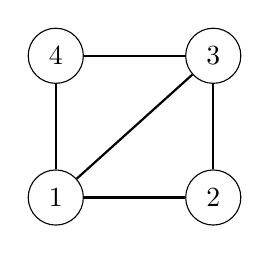
\begin{tikzpicture}[
  v/.style={circle, draw, minimum size=7mm},
  e/.style={thick}
]
\node[v] (1) at (0,0) {1};
\node[v] (2) at (2,0) {2};
\node[v] (3) at (2,1.8) {3};
\node[v] (4) at (0,1.8) {4};

% undirected edges
\draw[e] (1)--(2);
\draw[e] (2)--(3);
\draw[e] (3)--(4);
\draw[e] (4)--(1);
\draw[e] (1)--(3);
\end{tikzpicture}
\caption{Undirected graph on 4 nodes}
\label{fig:undirected4}
\end{subfigure}
\hfill
\begin{subfigure}[t]{0.45\textwidth}
\centering
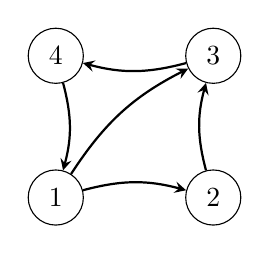
\begin{tikzpicture}[
  v/.style={circle, draw, minimum size=7mm},
  e/.style={thick, ->, >=stealth}
]
\node[v] (1) at (0,0) {1};
\node[v] (2) at (2,0) {2};
\node[v] (3) at (2,1.8) {3};
\node[v] (4) at (0,1.8) {4};

% directed edges
\draw[e] (1) to[bend left=15] (2);
\draw[e] (2) to[bend left=15] (3);
\draw[e] (3) to[bend left=15] (4);
\draw[e] (4) to[bend left=15] (1);
\draw[e] (1) to[bend left=15] (3);
\end{tikzpicture}
\caption{Directed graph on 4 nodes}
\label{fig:directed4}
\end{subfigure}

\caption{Examples of (a) undirected and (b) directed graphs on four nodes.}
\label{fig:two-graphs}
\end{figure}

\begin{tip}{Mutual edges}
    In directed graphs, it is possible for two nodes to have edges pointing to each other, known as \emph{mutual edges}. This indicates a bidirectional relationship between the nodes, such as mutual friendships on social media platforms.
\end{tip}

\subsubsection{Graph Types based on Edge properties}
\begin{itemize}[nosep]
    \item Simple graph: Graphs that do not contain self-loops (an edge connecting a node to itself) or multi-edges (multiple edges between the same two nodes). Most analysis focuses on simple graphs.
    \item Multigraph: Graphs that may contain self-loops and/or multi-edges. Multi-edges are often encoded as edge weights (counts).
    \item Weighted graph: Graphs where edges are labeled with numerical values. The length of a path in a weighted graph is the sum of weighted of the traversed edges.
\end{itemize}

% Preamble:
% \usepackage{tikz}
% \usepackage{subcaption}

\begin{figure}[ht]
\centering

% ---------------- (a) Simple graph ----------------
\begin{subfigure}[t]{0.47\textwidth}
\centering
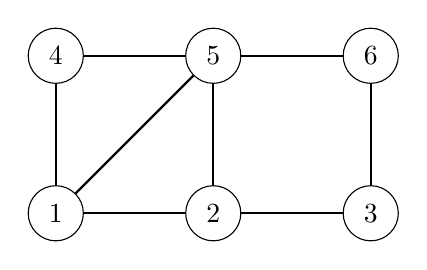
\begin{tikzpicture}[
  v/.style={circle, draw, minimum size=7mm},
  e/.style={thick}
]
% same 6 node positions for both subfigures
\node[v] (1) at (0,0) {1};
\node[v] (2) at (2,0) {2};
\node[v] (3) at (4,0) {3};
\node[v] (4) at (0,2) {4};
\node[v] (5) at (2,2) {5};
\node[v] (6) at (4,2) {6};

% simple graph edges (no loops, no parallel edges)
\draw[e] (1)--(2);
\draw[e] (2)--(3);
\draw[e] (1)--(4);
\draw[e] (2)--(5);
\draw[e] (3)--(6);
\draw[e] (4)--(5);
\draw[e] (5)--(6);
\draw[e] (1)--(5);

\end{tikzpicture}
\caption{Simple graph on 6 nodes}
\label{fig:simple6}
\end{subfigure}
\hfill
% ---------------- (b) Multigraph ----------------
\begin{subfigure}[t]{0.47\textwidth}
\centering
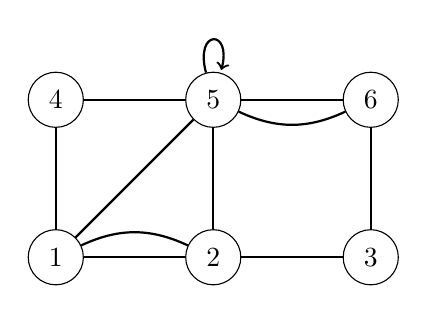
\begin{tikzpicture}[
  v/.style={circle, draw, minimum size=7mm},
  e/.style={thick}
]
% same 6 node positions
\node[v] (1) at (0,0) {1};
\node[v] (2) at (2,0) {2};
\node[v] (3) at (4,0) {3};
\node[v] (4) at (0,2) {4};
\node[v] (5) at (2,2) {5};
\node[v] (6) at (4,2) {6};

% base edges (same as simple graph, for comparison)
\draw[e] (1)--(2);
\draw[e] (2)--(3);
\draw[e] (1)--(4);
\draw[e] (2)--(5);
\draw[e] (3)--(6);
\draw[e] (4)--(5);
\draw[e] (5)--(6);
\draw[e] (1)--(5);

% parallel edges (multiedges)
\draw[e, bend left=25] (1) to (2);  % second edge between 1 and 2
\draw[e, bend right=25] (5) to (6); % second edge between 5 and 6

% a loop (allowed in many multigraph definitions)
\draw[e] (5) edge[loop above] (5);

\end{tikzpicture}
\caption{Multigraph on the same 6 nodes}
\label{fig:multi6}
\end{subfigure}

\caption{A simple graph versus a multigraph on the same vertex set. The multigraph includes parallel edges and a self-loop.}
\label{fig:simple-vs-multigraph}
\end{figure}


\begin{example}{Network Representations as Graphs}{ex:network-graph-representations}
    Different types of networks can be represented using various graph structures. For instance, the World Wide Web is often modeled as a directed multigraph with loops, while citation networks are directed and acyclic. Collaboration networks are typically undirected and unweighted. Table~\ref{tab:network-graph-representations} summarizes some common examples.
\end{example}
\begin{table}[ht]
\centering
\begin{tabular}{ll}
\toprule
\textbf{Network} & \textbf{Graph Representations} \\
\midrule
WWW & Directed multi-graph (with loops), unweighted \\
Citation Network & Directed, unweighted, acyclic \\
Collaboration Network & Undirected, unweighted \\
Mobile Phone Calls & Directed, weighted \\
Protein Interaction & Undirected multi-graph (with loops), unweighted \\
\bottomrule
\end{tabular}
\caption{Examples of networks and common graph representations.}
\label{tab:network-graph-representations}
\end{table}

\subsection{Local Connectivity and Degree}
\subsubsection{Adjacency and Incidence}
Two nodes are \emph{adjacent} if they are directly connected by an edge. The set of nodes adjacent to a given node $u$ is called the \emph{neighborhood} of $u$, denoted $N(u)$.

An edge is \emph{incident} to a node if the node is one of the edge's endpoints. For an edge $(u,v)$, it is incident to both $u$ and $v$. See Fig~\ref{fig:adjacency-incidence} for an illustration.

% Preamble:
% \usepackage{tikz}

\begin{figure}[ht]
\centering
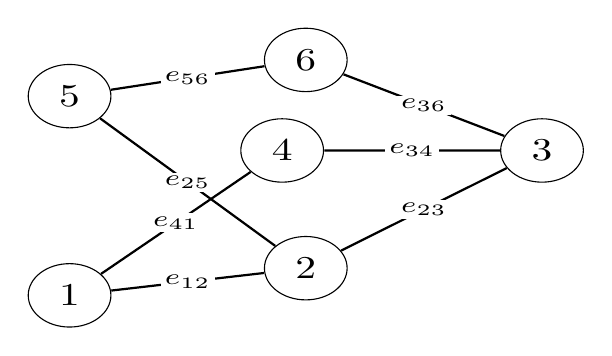
\begin{tikzpicture}[
    xscale=1.5, yscale=1.15, transform shape,
  v/.style={circle, draw, minimum size=7mm},
  e/.style={thick},
  elab/.style={midway, fill=white, inner sep=1pt, font=\scriptsize}
]
% --- 6 vertices (placed "randomly") ---
\node[v] (1) at (0,0)   {$1$};
\node[v] (2) at (2,0.3) {$2$};
\node[v] (3) at (4,1.6) {$3$};
\node[v] (4) at (1.8,1.6) {$4$};
\node[v] (5) at (0,2.2) {$5$};
\node[v] (6) at (2.0,2.6) {$6$};

% --- edges with labels e_{ij} ---
\draw[e] (1)-- node[elab] {$e_{12}$} (2);
\draw[e] (2)-- node[elab] {$e_{23}$} (3);
\draw[e] (3)-- node[elab] {$e_{34}$} (4);
\draw[e] (4)-- node[elab] {$e_{41}$} (1);
\draw[e] (2)-- node[elab] {$e_{25}$} (5);
\draw[e] (5)-- node[elab] {$e_{56}$} (6);
\draw[e] (3)-- node[elab] {$e_{36}$} (6);
\end{tikzpicture}

\caption{A simple undirected graph with vertex set $V=\{1,2,3,4,5,6\}$ and edge set
$E=\{e_{12},e_{23},e_{34},e_{41},e_{25},e_{56},e_{36}\}$.
\textbf{Adjacency (vertex--vertex):} vertices $1$ and $2$ are adjacent because $e_{12}$ joins them; vertices $1$ and $3$ are not adjacent because there is no edge between them.
\textbf{Incidence (edge--vertex):} edge $e_{12}$ is incident to vertices $1$ and $2$ (and is not incident to $3$); the edges incident to vertex $2$ are $e_{12}$, $e_{23}$, and $e_{25}$.}
\label{fig:adjacency-incidence}
\end{figure}


\subsubsection{Vertex degrees}
The \emph{degree} $(d_v)$ of a vertex $v$ is its number of incident edges. High-degree vertices are often considered influential, central, or prominent. See Fig~\ref{fig:degrees-example} for an illustration.

% Preamble:
% \usepackage{tikz}

\begin{figure}[ht]
\centering
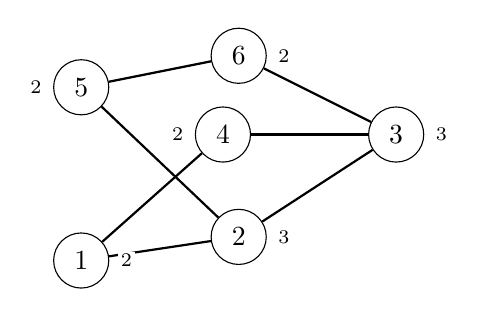
\begin{tikzpicture}[
  v/.style={circle, draw, minimum size=7mm},
  e/.style={thick},
  deg/.style={font=\scriptsize, fill=white, inner sep=1pt}
]
% --- 6 vertices (placed "randomly") ---
\node[v] (1) at (0,0)   {$1$};
\node[v] (2) at (2,0.3) {$2$};
\node[v] (3) at (4,1.6) {$3$};
\node[v] (4) at (1.8,1.6) {$4$};
\node[v] (5) at (0,2.2) {$5$};
\node[v] (6) at (2.0,2.6) {$6$};

% --- edges (no edge labels) ---
\draw[e] (1)--(2);
\draw[e] (2)--(3);
\draw[e] (3)--(4);
\draw[e] (4)--(1);
\draw[e] (2)--(5);
\draw[e] (5)--(6);
\draw[e] (3)--(6);

% --- degree annotations d(v) next to each vertex ---
\node[deg, anchor=west] at ([xshift=3pt]1.east) {$2$};
\node[deg, anchor=west] at ([xshift=3pt]2.east) {$3$};
\node[deg, anchor=west] at ([xshift=3pt]3.east) {$3$};
\node[deg, anchor=east] at ([xshift=-3pt]4.west) {$2$};
\node[deg, anchor=east] at ([xshift=-3pt]5.west) {$2$};
\node[deg, anchor=west] at ([xshift=3pt]6.east) {$2$};

\end{tikzpicture}

\caption{A simple undirected graph on $V=\{1,2,3,4,5,6\}$ with vertex degrees shown.
For example, $d(2)=3$ because vertex $2$ is adjacent to $\{1,3,5\}$, while $d(1)=2$ because vertex $1$ is adjacent to $\{2,4\}$.}
\label{fig:degrees-example}
\end{figure}


\begin{definition}{Neighborhood}{def:neighborhood}
The \emph{neighborhood} $\mathcal{N}_i$ of a node $i$ is the set of all its adjacent nodes.

The size of the neighborhood is equal to the degree, i.e., $|\mathcal{N}_i|=d_i$.
\end{definition}

\subsubsection{Degree formulas and properties}
The following properties hold for an undirected graph:
\begin{properties}{Degree Properties}{prop:degree-properties}
\begin{itemize}[nosep]
    \item Degree range: For any vertex $v$, $0 \leq d_v \leq n-1$, where $n$ is the total number of vertices in the graph.
    \item Sum of degrees: The sum of the degrees of all vertices is equal to twice the number of edges: \[\sum_{v=1}^{|V|} d_v = 2|E|.\]
    \item Odd degree count: The number of vertices with an odd degree must be an even number.
\end{itemize}
\end{properties}

\begin{proof}
Consider a finite undirected graph $G=(V,E)$ (allowing neither direction nor multiple counting beyond multiplicity).
Each edge $e=\{u,w\}\in E$ is incident to exactly two vertices, namely $u$ and $w$.

Now count the number of \emph{incidences} (vertex--edge pairs $(v,e)$ where $e$ is incident to $v$) in two ways:
\begin{itemize}
  \item Fix a vertex $v$. There are exactly $d(v)$ edges incident to $v$, so the total number of incidences is
  \(\sum_{v\in V} d(v)\).
  \item Fix an edge $e$. It contributes exactly $2$ incidences (one for each endpoint), so the total number of incidences is
  \(2|E|\).
\end{itemize}
Both expressions count the same set of incidences, hence
\[
\sum_{v\in V} d(v)=2|E|.
\]
\end{proof}

\subsubsection{Degrees in Directed Graphs}
In directed graphs (digraphs), vertices have two types of degrees:
\begin{itemize}[nosep]
    \item \textbf{In-degree} ($d_v^i$): the number of edges pointing \emph{to} vertex $v$.
    \item \textbf{Out-degree} ($d_v^o$): the number of edges pointing \emph{away} from vertex $v$.
\end{itemize}
% Preamble:
% \usepackage{tikz}
% \usepackage{xcolor}

\begin{figure}[ht]
\centering
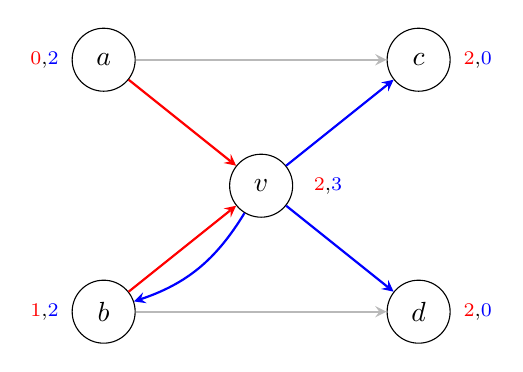
\begin{tikzpicture}[
  vtx/.style={circle, draw, minimum size=8mm},
  e/.style={->, thick, >=stealth},
  inE/.style={e, red},
  outE/.style={e, blue},
  otherE/.style={e, gray!55},
  deg/.style={font=\scriptsize, fill=white, inner sep=1pt}
]

% --- vertices ---
\node[vtx] (a) at (0, 1.6) {$a$};
\node[vtx] (b) at (0,-1.6) {$b$};
\node[vtx] (v) at (2, 0.0) {$v$};
\node[vtx] (c) at (4, 1.6) {$c$};
\node[vtx] (d) at (4,-1.6) {$d$};

% --- edges ---
% incoming to v (red)
\draw[inE] (a) -- (v);
\draw[inE] (b) -- (v);

% outgoing from v (blue)
\draw[outE] (v) -- (c);
\draw[outE] (v) -- (d);
\draw[outE] (v) to[bend left=20] (b);

% other edges (gray) for context
\draw[otherE] (a) -- (c);
\draw[otherE] (b) -- (d);

% --- (in-degree, out-degree) labels next to each vertex ---
% format: (red in-degree, blue out-degree)
\node[deg] at (-0.75, 1.6) {\textcolor{red}{0},\textcolor{blue}{2}}; % a: out to v and c
\node[deg] at (-0.75,-1.6) {\textcolor{red}{1},\textcolor{blue}{2}}; % b: in from v; out to v and d
\node[deg] at ( 2.85, 0.0) {\textcolor{red}{2},\textcolor{blue}{3}}; % v: in from a,b; out to c,d,b
\node[deg] at ( 4.75, 1.6) {\textcolor{red}{2},\textcolor{blue}{0}}; % c: in from v and a
\node[deg] at ( 4.75,-1.6) {\textcolor{red}{2},\textcolor{blue}{0}}; % d: in from v and b

\end{tikzpicture}
\caption{A directed graph where each vertex is annotated with its \textcolor{red}{in-degree} and \textcolor{blue}{out-degree} as an ordered pair \((d^{-},d^{+})\). Incoming edges are shown in \textcolor{red}{red} and outgoing edges in \textcolor{blue}{blue}.}
\label{fig:in-out-degree-pairs}
\end{figure}


\subsection{Global connectivity and Path}
\subsubsection{Movement in a Graph}

\begin{definition}{Path, Walk, Cycle}{def:path-walk-cycle}
A \emph{path} in a graph is a consecutive sequence of distinct vertices $\{v_0, v_1, \dots, v_l\}$ such that $v_i$ and $v_{i+1}$ are adjacent. The length of the path is $l$.

A \emph{walk} is similar to a path, but vertices and edges can be repeated. A walk that starts and ends at the same vertex is called a \emph{closed walk}, or a \emph{cycle} if no other vertices are repeated. 
\end{definition}
These definition generalize naturally to directed graphs.

% Preamble:
% \usepackage{tikz}
% \usepackage{xcolor}

\begin{figure}[ht]
\centering
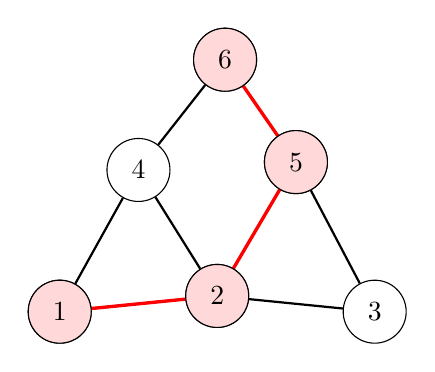
\begin{tikzpicture}[
  v/.style={circle, draw, minimum size=8mm},
  e/.style={thick},
  pathE/.style={very thick, red},
  pathV/.style={circle, draw, fill=red!15, minimum size=8mm}
]

% --- vertices ---
\node[v] (1) at (0,0)   {$1$};
\node[v] (2) at (2,0.2) {$2$};
\node[v] (3) at (4,0.0) {$3$};
\node[v] (4) at (1.0,1.8) {$4$};
\node[v] (5) at (3.0,1.9) {$5$};
\node[v] (6) at (2.1,3.2) {$6$};

% --- edges (graph) ---
\draw[e] (1)--(2);
\draw[e] (2)--(3);
\draw[e] (1)--(4);
\draw[e] (2)--(4);
\draw[e] (2)--(5);
\draw[e] (3)--(5);
\draw[e] (4)--(6);
\draw[e] (5)--(6);

% --- highlighted path: 1-2-5-6 ---
\draw[pathE] (1)--(2);
\draw[pathE] (2)--(5);
\draw[pathE] (5)--(6);

% highlight the path vertices (optional)
\node[pathV] at (1) {$1$};
\node[pathV] at (2) {$2$};
\node[pathV] at (5) {$5$};
\node[pathV] at (6) {$6$};

\end{tikzpicture}
\caption{A graph with the path $1 \to 2 \to 5 \to 6$ highlighted in red.}
\label{fig:path-highlight}
\end{figure}


\subsubsection{Distance and Diameter}
\begin{definition}{Distance and Diameter}{def:distance-diameter}
The \emph{distance} between two vertices $u$ and $v$, denoted $d(u,v)$, is the length of the shortest path connecting them. If no path exists, the distance is defined to be infinite.

\emph{Diameter} of a graph is the maximum distance between any pair of vertices in the graph:
\[\text{diameter}(G) = \max_{u,v \in V} d(u,v).\]
\end{definition}

Efficient algorithms exist for computing shortest paths in both undirected and directed graphs, such as Dijkstra's algorithm for graphs with non-negative edge weights, Floyd-Warshall algorithm for dense graphs, and Bellman-Ford algorithm for graphs with negative edge weights.

\subsubsection{Connectivity}
Vertex $v$ is \emph{reachable} from vertex $u$ if there exists a path from $u$ to $v$.

\begin{definition}{Connected graphs (Undirected)}{def:connected-graphs-undirected}
A graph is \emph{connected} if every vertex is reachable from every other vertex. Removing a ``bridge edge'' (an edge whose removal increases the number of connected components) can disconnect the graph.
\end{definition}
% Preamble:
% \usepackage{tikz}
% \usepackage{xcolor}

\begin{figure}[ht]
\centering
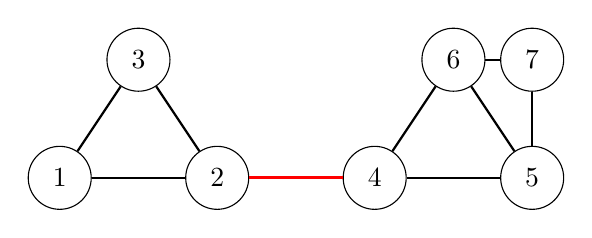
\begin{tikzpicture}[
  v/.style={circle, draw, minimum size=8mm},
  e/.style={thick},
  bridge/.style={very thick, red}
]

% --- vertices ---
\node[v] (1) at (0,0)   {$1$};
\node[v] (2) at (2,0)   {$2$};
\node[v] (3) at (1,1.5) {$3$};

\node[v] (4) at (4,0)   {$4$};
\node[v] (5) at (6,0)   {$5$};
\node[v] (6) at (5,1.5) {$6$};
\node[v] (7) at (6,1.5) {$7$};

% --- edges (connected graph) ---
% left triangle
\draw[e] (1)--(2);
\draw[e] (2)--(3);
\draw[e] (3)--(1);

% right cluster
\draw[e] (4)--(5);
\draw[e] (4)--(6);
\draw[e] (5)--(6);
\draw[e] (6)--(7);
\draw[e] (5)--(7);

% bridge edge (removing it disconnects the graph)
\draw[bridge] (2)--(4);

\end{tikzpicture}
\caption{A connected undirected graph on 7 vertices. The red edge $(2,4)$ is a \emph{bridge}: removing it disconnects the graph into two components (the triangle on $\{1,2,3\}$ and the subgraph on $\{4,5,6,7\}$).}
\label{fig:bridge-example}
\end{figure}

\begin{definition}{Connected components}{def:connected-components}
A \emph{component} is a maximally connected subgraph. A maximal subgraph is one where adding any other vertex would ruin the connectivity. Disconnected graphs have two or more components.
\end{definition}
% Preamble:
% \usepackage{tikz}
% \usepackage{xcolor}

\begin{figure}[ht]
\centering
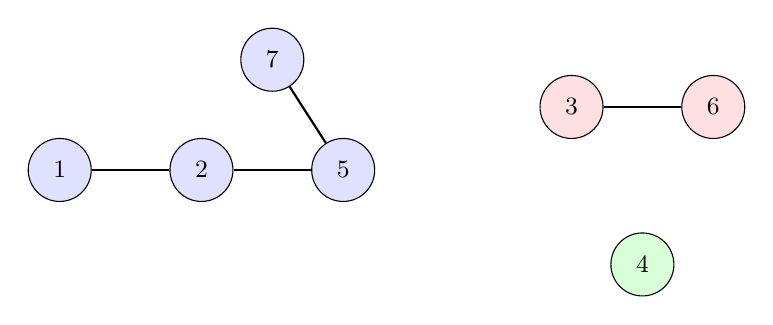
\begin{tikzpicture}[
  v/.style={circle, draw, minimum size=8mm, font=\small},
  blueV/.style={v, fill=blue!12},
  redV/.style={v, fill=red!12},
  greenV/.style={v, fill=green!15},
  e/.style={thick}
]

% --- Component C1 = {1,2,5,7} (blue) ---
\node[blueV] (1) at (0,0)   {1};
\node[blueV] (2) at (1.8,0) {2};
\node[blueV] (5) at (3.6,0) {5};
\node[blueV] (7) at (2.7,1.4) {7};

\draw[e] (1)--(2);
\draw[e] (2)--(5);
\draw[e] (5)--(7);

% --- Component C2 = {3,6} (red) ---
\node[redV] (3) at (6.5,0.8) {3};
\node[redV] (6) at (8.3,0.8) {6};
\draw[e] (3)--(6);

% --- Component C3 = {4} (green, isolated) ---
\node[greenV] (4) at (7.4,-1.2) {4};

\end{tikzpicture}
\caption{A disconnected graph with three connected components:
\textcolor{blue}{$\{1,2,5,7\}$}, \textcolor{red}{$\{3,6\}$}, and \textcolor{green}{$\{4\}$}.
The subgraph on $\{3,4,6\}$ is not connected because vertex $4$ is isolated from $\{3,6\}$, while the subgraph on $\{1,2,5\}$ is not maximal since it can be enlarged to the connected component $\{1,2,5,7\}$.}
\label{fig:components-example}
\end{figure}

Disconnected graphs have 2 or more components, largest component often called giant component. Large real-world networks often exhibit one giant component.

\begin{tip}{Why do we expect to find a single giant component?}{tip:giant-component}
    In many real-world networks, the presence of a single giant component can be attributed to the underlying connectivity patterns and the nature of interactions among nodes. Factors such as preferential attachment, where new nodes are more likely to connect to already well-connected nodes, and the small-world phenomenon, where most nodes can be reached from every other by a small number of steps, contribute to the formation of a giant component. Additionally, real-world networks often exhibit clustering and community structures that facilitate connectivity within the giant component.
\end{tip}

\subsubsection{Connectivity in Directed Graphs}

Connectivity is more complex in directed graphs and has two main notions:
\begin{enumerate}
    \item Strongly connected: A digraph is strongly connected if for every pair of vertices $u$ and $v$, $u$ is reachable from $v$ (via a directed path) and $v$ is reachable from $u$. 
    \item Weakly connected: A digraph is weakly connected if it remains connected after disregarding the edge directions (i.e., its underlying undirected graph is connected). Strongly connectivity implies weak connectivity.
\end{enumerate}

% Preamble:
% \usepackage{tikz}
% \usetikzlibrary{fit, backgrounds}

\begin{figure}[ht]
\centering
\begin{tikzpicture}[
  v/.style={circle, draw, minimum size=8mm, font=\small},
  e/.style={->, thick, >=stealth}
]

% --- vertices ---
\node[v] (1) at (0,0) {1};
\node[v] (2) at (2,0) {2};
\node[v] (3) at (4,0) {3};
\node[v] (4) at (6,0) {4};
\node[v] (5) at (8,0) {5};
\node[v] (6) at (10,0) {6};

% --- edges (directed) ---
% SCC1: {1,2,3}
\draw[e] (1) -- (2);
\draw[e] (2) -- (3);
\draw[e, bend left=35] (3) to (1);

% SCC2: {4,5}
\draw[e] (4) -- (5);
\draw[e, bend left=35] (5) to (4);

% links between SCCs (make the graph weakly connected, but not strongly)
\draw[e] (3) -- (4);
\draw[e] (5) -- (6);

% --- highlight strongly connected components (background boxes) ---
\begin{scope}[on background layer]
  \node[draw, rounded corners, fill=blue!12, inner sep=6pt,
        fit=(1)(2)(3)] {};
  \node[draw, rounded corners, fill=green!12, inner sep=6pt,
        fit=(4)(5)] {};
  \node[draw, rounded corners, fill=orange!12, inner sep=6pt,
        fit=(6)] {};
\end{scope}

\end{tikzpicture}

\caption{A directed graph that is \emph{weakly connected} (ignoring arrow directions, all vertices lie in one connected component) but \emph{not strongly connected} (there is no directed path from $6$ back to earlier vertices, and no directed path from $\{4,5\}$ back to $\{1,2,3\}$). The strongly connected components are highlighted: \textcolor{blue}{$\{1,2,3\}$}, \textcolor{green}{$\{4,5\}$}, and \textcolor{orange}{$\{6\}$}.}
\label{fig:weak-not-strong}
\end{figure}


\subsection{Specialized Graph Structures}
\subsubsection{Complete Graphs and Cliques}
A \emph{complete graph} is a simple undirected graph in which every pair of distinct vertices is connected by a unique edge.

% Preamble:
% \usepackage{tikz}
% \usepackage{subcaption}

\begin{figure}[ht]
\centering

\begin{subfigure}[t]{0.22\textwidth}
\centering
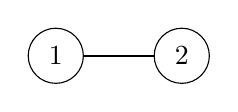
\begin{tikzpicture}[v/.style={circle,draw,minimum size=7mm}, e/.style={thick}]
\node[v] (1) at (0,0) {1};
\node[v] (2) at (1.6,0) {2};
\draw[e] (1)--(2);
\end{tikzpicture}
\caption{$K_2$}
\end{subfigure}
\hfill
\begin{subfigure}[t]{0.22\textwidth}
\centering
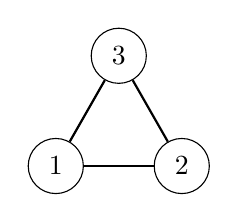
\begin{tikzpicture}[v/.style={circle,draw,minimum size=7mm}, e/.style={thick}]
\node[v] (1) at (0,0) {1};
\node[v] (2) at (1.6,0) {2};
\node[v] (3) at (0.8,1.4) {3};
\draw[e] (1)--(2);
\draw[e] (2)--(3);
\draw[e] (3)--(1);
\end{tikzpicture}
\caption{$K_3$}
\end{subfigure}
\hfill
\begin{subfigure}[t]{0.22\textwidth}
\centering
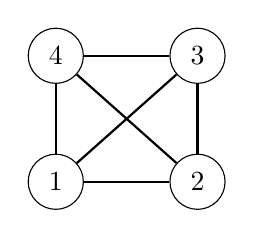
\begin{tikzpicture}[v/.style={circle,draw,minimum size=7mm}, e/.style={thick}]
\node[v] (1) at (0,0) {1};
\node[v] (2) at (1.8,0) {2};
\node[v] (3) at (1.8,1.6) {3};
\node[v] (4) at (0,1.6) {4};
\draw[e] (1)--(2);
\draw[e] (2)--(3);
\draw[e] (3)--(4);
\draw[e] (4)--(1);
\draw[e] (1)--(3);
\draw[e] (2)--(4);
\end{tikzpicture}
\caption{$K_4$}
\end{subfigure}
\hfill
\begin{subfigure}[t]{0.22\textwidth}
\centering
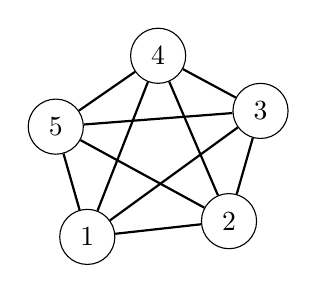
\begin{tikzpicture}[v/.style={circle,draw,minimum size=7mm}, e/.style={thick}]
\node[v] (1) at (0,0) {1};
\node[v] (2) at (1.8,0.2) {2};
\node[v] (3) at (2.2,1.6) {3};
\node[v] (4) at (0.9,2.3) {4};
\node[v] (5) at (-0.4,1.4) {5};
\draw[e] (1)--(2);
\draw[e] (1)--(3);
\draw[e] (1)--(4);
\draw[e] (1)--(5);
\draw[e] (2)--(3);
\draw[e] (2)--(4);
\draw[e] (2)--(5);
\draw[e] (3)--(4);
\draw[e] (3)--(5);
\draw[e] (4)--(5);
\end{tikzpicture}
\caption{$K_5$}
\end{subfigure}

\caption{Complete graphs $K_n$ for $n=2,3,4,5$.}
\label{fig:complete-k2-k5}
\end{figure}


\begin{properties}{Number of edges in complete graphs}{prop:complete-graph-edges}
The number of edges is equal to the number of vertex pairs:
\[
\text{Number of edges in }K_n=\binom{n}{2}=\frac{n(n-1)}{2}
\]
\end{properties}
\begin{proof}
In the complete graph $K_n$, every pair of distinct vertices is connected by exactly one edge.
Thus, counting edges is the same as counting unordered pairs of distinct vertices.

The number of ways to choose 2 vertices from $n$ (order does not matter) is
\[
\binom{n}{2}=\frac{n(n-1)}{2}.
\]
Therefore $|E(K_n)|=\binom{n}{2}=\frac{n(n-1)}{2}$.
\end{proof}

A \emph{clique} in a graph is a subset of vertices such that every two distinct vertices are adjacent. In other words, a clique is a complete subgraph. The size of the largest clique in a graph is called the \emph{clique number}.

% Preamble:
% \usepackage{tikz}

\begin{figure}[ht]
\centering
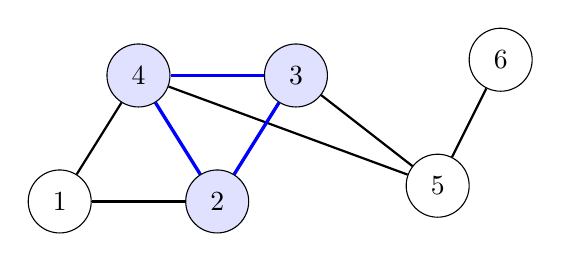
\begin{tikzpicture}[
  v/.style={circle, draw, minimum size=8mm},
  e/.style={thick},
  cliqueV/.style={circle, draw, fill=blue!12, minimum size=8mm},
  cliqueE/.style={very thick, blue}
]

% vertices
\node[v] (1) at (0,0) {1};
\node[cliqueV] (2) at (2,0) {2};
\node[cliqueV] (3) at (3,1.6) {3};
\node[cliqueV] (4) at (1,1.6) {4};
\node[v] (5) at (4.8,0.2) {5};
\node[v] (6) at (5.6,1.8) {6};

% edges (graph)
\draw[e] (1)--(2);
\draw[e] (1)--(4);
\draw[e] (2)--(4);
\draw[e] (2)--(3);
\draw[e] (3)--(4);
\draw[e] (3)--(5);
\draw[e] (5)--(6);
\draw[e] (4)--(5);

% highlight a clique (here: {2,3,4} is a 3-clique)
\draw[cliqueE] (2)--(3);
\draw[cliqueE] (3)--(4);
\draw[cliqueE] (2)--(4);

\end{tikzpicture}
\caption{An example of a clique: vertices $\{2,3,4\}$ form a 3-clique (a $K_3$ subgraph), since every pair among them is connected by an edge.}
\label{fig:clique-example}
\end{figure}


\subsubsection{Regular graphs}

A \emph{regular graph} is a graph where every vertex has the same degree $k$. Such a graph is called a $k$-regular graph.

The complete graph $K_n$ is an example of a $(n-1)$-regular graph, since every vertex is connected to all other $n-1$ vertices. Cycles are examples of 2-regular graphs, as each vertex is connected to exactly two other vertices.

% Preamble:
% \usepackage{tikz}
% \usepackage{subcaption}

\begin{figure}[ht]
\centering

\begin{subfigure}[t]{0.32\textwidth}
\centering
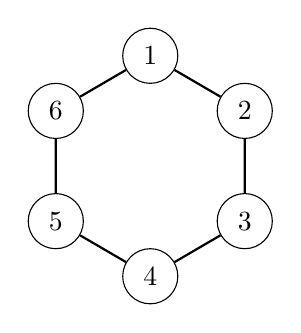
\begin{tikzpicture}[
  v/.style={circle, draw, minimum size=7mm},
  e/.style={thick}
]
\node[v] (1) at (0,1.4) {1};
\node[v] (2) at (1.2,0.7) {2};
\node[v] (3) at (1.2,-0.7) {3};
\node[v] (4) at (0,-1.4) {4};
\node[v] (5) at (-1.2,-0.7) {5};
\node[v] (6) at (-1.2,0.7) {6};
\draw[e] (1)--(2)--(3)--(4)--(5)--(6)--(1);
\end{tikzpicture}
\caption{$C_6$ (2-regular)}
\end{subfigure}
\hfill
\begin{subfigure}[t]{0.32\textwidth}
\centering
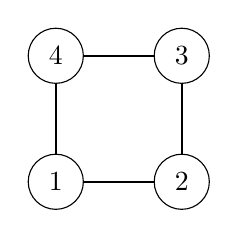
\begin{tikzpicture}[
  v/.style={circle, draw, minimum size=7mm},
  e/.style={thick}
]
\node[v] (1) at (0,0) {1};
\node[v] (2) at (1.6,0) {2};
\node[v] (3) at (1.6,1.6) {3};
\node[v] (4) at (0,1.6) {4};
\draw[e] (1)--(2)--(3)--(4)--(1);
\end{tikzpicture}
\caption{$C_4$ (2-regular)}
\end{subfigure}
\hfill
\begin{subfigure}[t]{0.32\textwidth}
\centering
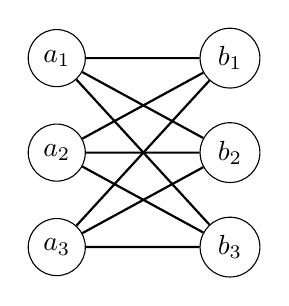
\begin{tikzpicture}[
  v/.style={circle, draw, minimum size=7mm},
  e/.style={thick}
]
\node[v] (a1) at (0, 1.2) {$a_1$};
\node[v] (a2) at (0, 0.0) {$a_2$};
\node[v] (a3) at (0,-1.2) {$a_3$};

\node[v] (b1) at (2.2, 1.2) {$b_1$};
\node[v] (b2) at (2.2, 0.0) {$b_2$};
\node[v] (b3) at (2.2,-1.2) {$b_3$};

\draw[e] (a1)--(b1) (a1)--(b2) (a1)--(b3);
\draw[e] (a2)--(b1) (a2)--(b2) (a2)--(b3);
\draw[e] (a3)--(b1) (a3)--(b2) (a3)--(b3);
\end{tikzpicture}
\caption{$K_{3,3}$ (3-regular)}
\end{subfigure}

\caption{Examples of regular graphs: $C_6$ and $C_4$ are 2-regular; $K_{3,3}$ is 3-regular.}
\label{fig:regular-examples}
\end{figure}

Regular graphs frequently arise in the study of crystal structures (physics/chemistry), pixel adjacency models in image processing (geo-spatial settings), and modeling opinion formation or information cycles.

\subsubsection{Trees and Acyclic Graphs}
\begin{definition}
{Trees and Forests}{def:trees-forests}
A connected graph that is acyclic (contains no cycles) is called a \emph{tree}. 

A \emph{forest} is a disjoint set of trees.
\end{definition}


A \emph{directed tree} (or \emph{arborescence}) is a directed graph where there is a unique directed path from a designated root node to every other node. 

\begin{definition}
{Directed Acyclic Graph (DAG)}{def:directed-acyclic-graph}
A \emph{directed acyclic graph} (DAG) is a directed graph with no directed cycles. The underlying graph of a DAG need not be a tree. DAGs are commonly used to represent hierarchical structures, such as task scheduling or data processing pipelines.
\end{definition}

% Preamble:
% \usepackage{tikz}
% \usepackage{subcaption}

\begin{figure}[ht]
\centering

% ---------------- (a) Tree ----------------
\begin{subfigure}[t]{0.48\textwidth}
\centering
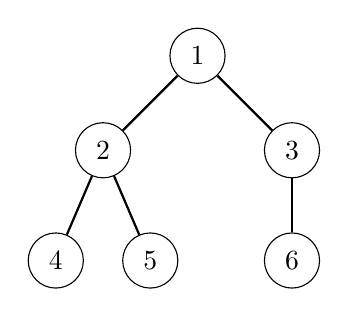
\begin{tikzpicture}[
  v/.style={circle, draw, minimum size=7mm},
  e/.style={thick}
]
\node[v] (1) at (0,0) {1};
\node[v] (2) at (-1.2,-1.2) {2};
\node[v] (3) at (1.2,-1.2) {3};
\node[v] (4) at (-1.8,-2.6) {4};
\node[v] (5) at (-0.6,-2.6) {5};
\node[v] (6) at (1.2,-2.6) {6};

\draw[e] (1)--(2);
\draw[e] (1)--(3);
\draw[e] (2)--(4);
\draw[e] (2)--(5);
\draw[e] (3)--(6);
\end{tikzpicture}
\caption{Tree}
\label{fig:tree}
\end{subfigure}
\hfill
% ---------------- (b) Forest ----------------
\begin{subfigure}[t]{0.48\textwidth}
\centering
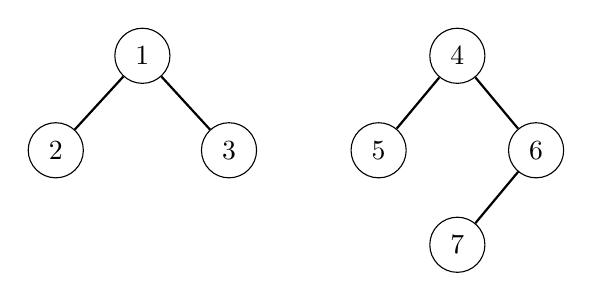
\begin{tikzpicture}[
  v/.style={circle, draw, minimum size=7mm},
  e/.style={thick}
]
% Tree 1
\node[v] (1) at (0,0) {1};
\node[v] (2) at (-1.1,-1.2) {2};
\node[v] (3) at (1.1,-1.2) {3};
\draw[e] (1)--(2);
\draw[e] (1)--(3);

% Tree 2 (disjoint)
\node[v] (4) at (4,0) {4};
\node[v] (5) at (3.0,-1.2) {5};
\node[v] (6) at (5.0,-1.2) {6};
\node[v] (7) at (4.0,-2.4) {7};
\draw[e] (4)--(5);
\draw[e] (4)--(6);
\draw[e] (6)--(7);
\end{tikzpicture}
\caption{Forest (disjoint trees)}
\label{fig:forest}
\end{subfigure}

\vspace{6mm}

% ---------------- (c) Directed tree / arborescence ----------------
\begin{subfigure}[t]{0.48\textwidth}
\centering
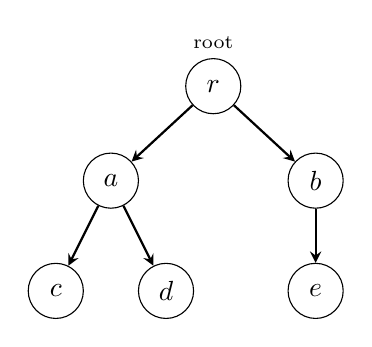
\begin{tikzpicture}[
  v/.style={circle, draw, minimum size=7mm},
  e/.style={->, thick, >=stealth}
]
\node[v] (r) at (0,0) {$r$};
\node[v] (a) at (-1.3,-1.2) {$a$};
\node[v] (b) at (1.3,-1.2) {$b$};
\node[v] (c) at (-2.0,-2.6) {$c$};
\node[v] (d) at (-0.6,-2.6) {$d$};
\node[v] (e1) at (1.3,-2.6) {$e$};

\draw[e] (r) -- (a);
\draw[e] (r) -- (b);
\draw[e] (a) -- (c);
\draw[e] (a) -- (d);
\draw[e] (b) -- (e1);

% root label
\node[draw=none, font=\scriptsize] at (0,0.55) {root};
\end{tikzpicture}
\caption{Directed tree (arborescence)}
\label{fig:arborescence}
\end{subfigure}
\hfill
% ---------------- (d) DAG ----------------
\begin{subfigure}[t]{0.48\textwidth}
\centering
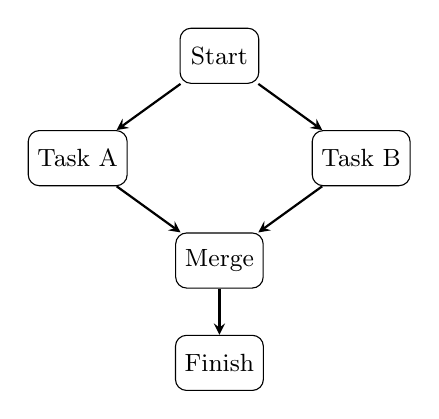
\begin{tikzpicture}[
  v/.style={rectangle, draw, rounded corners, minimum width=10mm, minimum height=7mm, font=\small},
  e/.style={->, thick, >=stealth}
]
\node[v] (s) at (0,0) {Start};
\node[v] (x) at (-1.8,-1.3) {Task A};
\node[v] (y) at (1.8,-1.3) {Task B};
\node[v] (z) at (0,-2.6) {Merge};
\node[v] (t) at (0,-3.9) {Finish};

\draw[e] (s) -- (x);
\draw[e] (s) -- (y);
\draw[e] (x) -- (z);
\draw[e] (y) -- (z);
\draw[e] (z) -- (t);
\end{tikzpicture}
\caption{DAG (no directed cycles)}
\label{fig:dag}
\end{subfigure}

\caption{Examples: (a) a tree (connected and acyclic), (b) a forest (disjoint set of trees), (c) a directed tree/arborescence (unique directed path from root to each node), and (d) a DAG (directed acyclic graph).}
\label{fig:tree-forest-arborescence-dag}
\end{figure}


\begin{example}
{Hierarchical Structures as Trees and DAGs}{ex:hierarchical-structures-trees-dags}
Hierarchical structures, such as organizational charts or file directory systems, can be effectively modeled using trees and DAGs. In an organizational chart, each employee reports to a single manager, forming a tree structure. In a file directory system, folders can contain subfolders and files, creating a DAG where cycles are avoided to prevent infinite loops in navigation.
\end{example}

